\documentclass{article}
\usepackage{amsmath, amssymb, amsfonts, amsthm}
\usepackage{xcolor}
\usepackage{tikz}
\usetikzlibrary{calc}
\usetikzlibrary{arrows.meta}

\begin{document}

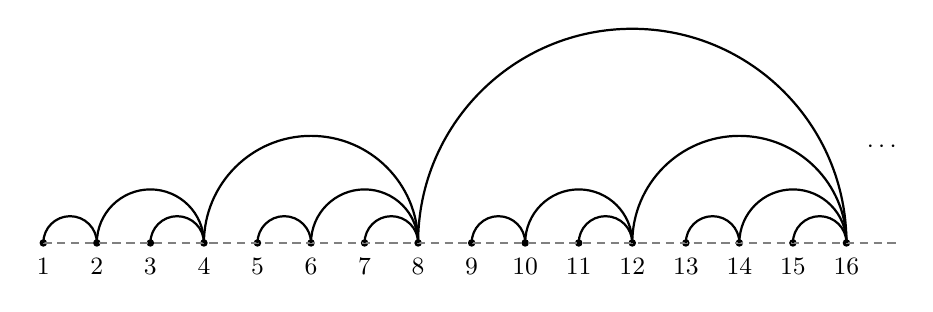
\begin{tikzpicture}[baseline=(current bounding box.center), scale=0.68,
    dot/.style={circle,fill,inner sep=1.5pt},
    every node/.style={font=\small}
]
    % Nodes 
    \foreach \i in {1,...,16}{
        \coordinate (P\i) at (\i,0);
        \fill (P\i) circle (2pt);
        \node[below=2pt] at (P\i) {\i};
    }

    \coordinate (P17) at (17,0);

    % Baseline
    \draw[line width=0.8pt, color=gray, densely dashed] (P1) -- (P17);

    \draw[line width=0.8pt]
        (P8) arc[start angle=180,end angle=0,radius=4];

    \foreach \b in {8,16}{
        \pgfmathtruncatemacro{\a}{\b-4}
        \draw[line width=0.8pt]
            (P\a) arc[start angle=180,end angle=0,radius=2];
    }

    % Self-dual bridges on the four size-4 blocks
    \foreach \b in {4,8,12,16}{
        \pgfmathtruncatemacro{\a}{\b-2}
        \draw[line width=0.8pt]
            (P\a) arc[start angle=180,end angle=0,radius=1];
    }

    % Self-dual bridges on the eight size-2 blocks
    \foreach \b in {2,4,6,8,10,12,14,16}{
        \pgfmathtruncatemacro{\a}{\b-1}
        \draw[line width=0.8pt]
            (P\a) arc[start angle=180,end angle=0,radius=0.5];
    }
    
    \node[draw=none, fill=white, inner sep=1.5pt] at (16.7, 1.8) {$\cdots$};
\end{tikzpicture}

\end{document}